\documentclass[11pt,a4paper]{article}
\usepackage[utf8]{inputenc}
\usepackage[T1]{fontenc}
\usepackage[margin=2cm]{geometry}
\usepackage{amsmath,amssymb}
\usepackage{siunitx}
\sisetup{per-mode=symbol}
\usepackage{booktabs}
\usepackage{array}
\usepackage{float}
\usepackage{xcolor}
\usepackage{listings}
\usepackage{hyperref}
\usepackage{enumitem}
\usepackage{fancyhdr}
\usepackage{tikz}

% ---- Couleurs ----
\definecolor{codegreen}{RGB}{40,140,60}
\definecolor{codegray}{RGB}{100,100,100}
\definecolor{codeblue}{RGB}{30,90,180}
\definecolor{codebg}{RGB}{248,248,248}
\definecolor{addgreen}{RGB}{230,255,230}
\definecolor{modblue}{RGB}{230,240,255}

% ---- Listings ----
\lstdefinestyle{cpp}{
  language=C++,
  backgroundcolor=\color{codebg},
  basicstyle=\small\ttfamily,
  keywordstyle=\color{codeblue}\bfseries,
  commentstyle=\color{codegreen}\itshape,
  stringstyle=\color{codegray},
  breaklines=true,
  frame=single,
  rulecolor=\color{gray!30},
  numbers=left,
  numberstyle=\tiny\color{gray},
  numbersep=5pt,
  tabsize=4,
  showstringspaces=false,
  morekeywords={G4bool,G4int,G4double,G4String,G4ThreeVector,MyTrackInfo,
                G4VUserTrackInformation,G4Step,G4Track,G4VProcess,
                G4LogicalVolume,G4AnalysisManager,G4AutoLock},
}

\lstdefinestyle{root}{
  language=C++,
  backgroundcolor=\color{codebg},
  basicstyle=\small\ttfamily,
  keywordstyle=\color{codeblue}\bfseries,
  frame=single,
  rulecolor=\color{gray!30},
  showstringspaces=false,
}

% ---- En-tete ----
\pagestyle{fancy}
\fancyhf{}
\fancyhead[L]{\small\textit{Modifications code Geant4 -- Tracking Compton dans le c\^one}}
\fancyhead[R]{\small\thepage}
\renewcommand{\headrulewidth}{0.4pt}

\begin{document}

% ===================================================================
%  TITRE
% ===================================================================
\begin{center}
{\LARGE\bfseries Synth\`ese des modifications du code Geant4}\\[6pt]
{\Large Diff\'erenciation des primaires directs\\
 et des primaires redirig\'es par diffusion Compton}\\[12pt]
{\large Simulation MiniX -- C\^one concentrateur en graphite}\\[8pt]
\today
\end{center}

\vspace{8pt}
\hrule
\vspace{12pt}

% ===================================================================
%  1. CONTEXTE ET MOTIVATION
% ===================================================================
\section{Contexte et motivation}

Dans Geant4, lorsqu'un photon $\gamma$ primaire subit une diffusion Compton,
le \textbf{photon diffus\'e continue comme le m\^eme track}
(m\^eme \texttt{trackID}, \texttt{parentID~=~0}).
Seul l'\'electron de recul est cr\'e\'e en tant que secondaire
(\texttt{creator\_process~=~"compt"}).

\medskip

Cons\'equence : au ScorePlane ($z = 18$~mm), un photon redirig\'e par Compton
dans le c\^one graphite est \textbf{indiscernable} d'un photon transmis
directement \`a travers le canal.
Les deux apparaissent comme \texttt{parentID~=~0},
\texttt{creator\_process~=~"primary"}.

\medskip

\textbf{Objectif :} ajouter un marquage (flag) sur le track primaire pour
distinguer les trois populations au ScorePlane :

\begin{center}
\renewcommand{\arraystretch}{1.2}
\begin{tabular}{clcc}
\toprule
\textbf{Cat.} & \textbf{Description} & \texttt{parentID} & \texttt{compton\_in\_cone} \\
\midrule
A & Primaire transmis directement        & 0 & 0 \\
B & Primaire redirig\'e par Compton      & 0 & 1 \\
C & Secondaire (e$^-$, $\gamma$ Brem\dots) & $\geq 1$ & --- \\
\bottomrule
\end{tabular}
\end{center}

% ===================================================================
%  2. FICHIERS MODIFIES
% ===================================================================
\section{Fichiers modifi\'es}

\begin{center}
\renewcommand{\arraystretch}{1.2}
\begin{tabular}{lll}
\toprule
\textbf{Fichier} & \textbf{R\'epertoire} & \textbf{Nature de la modification} \\
\midrule
\texttt{MyTrackInfo.hh}         & \texttt{include/} & Ajout champs Compton \\
\texttt{MyTrackInfo.cc}         & \texttt{src/}     & Initialisation des nouveaux champs \\
\texttt{SteppingAction.cc}      & \texttt{src/}     & D\'etection Compton dans le c\^one \\
\texttt{AnalysisManagerSetup.cc}& \texttt{src/}     & 5 nouvelles colonnes ntuple \\
\texttt{SurfaceSpectrumSD.cc}   & \texttt{src/}     & Lecture flag + remplissage ntuple \\
\bottomrule
\end{tabular}
\end{center}

\medskip

Aucun autre fichier n'est modifi\'e.
Les fichiers \texttt{.hh} et \texttt{.cc} non list\'es ci-dessus restent inchang\'es.

% ===================================================================
%  3. DETAIL DES MODIFICATIONS
% ===================================================================
\section{D\'etail des modifications}

% --- 3.1 MyTrackInfo ---
\subsection{\texttt{MyTrackInfo.hh / .cc} --- Stockage de l'information Compton}

Quatre nouveaux champs priv\'es sont ajout\'es \`a la classe \texttt{MyTrackInfo}
(qui h\'erite de \texttt{G4VUserTrackInformation} et est attach\'ee \`a chaque track) :

\begin{center}
\renewcommand{\arraystretch}{1.15}
{\small
\begin{tabular}{llll}
\toprule
\textbf{Champ} & \textbf{Type} & \textbf{Init.} & \textbf{Description} \\
\midrule
\texttt{fComptonInCone}   & \texttt{G4bool}        & \texttt{false}       & Flag : $\geq 1$ Compton dans le c\^one \\
\texttt{fNComptonInCone}  & \texttt{G4int}         & \texttt{0}           & Nombre total de Compton dans le c\^one \\
\texttt{fLastComptonPos}  & \texttt{G4ThreeVector} & \texttt{(0,0,0)}     & Position de la derni\`ere diffusion \\
\texttt{fLastComptonEkin} & \texttt{G4double}      & \texttt{0.}          & $E_{\mathrm{kin}}$ avant la derni\`ere diffusion \\
\bottomrule
\end{tabular}
}
\end{center}

\medskip

Accesseurs publics correspondants :
\texttt{Set/Get/Has} + \texttt{IncrementNComptonInCone()}.

L'include \texttt{G4ThreeVector.hh} est ajout\'e en en-t\^ete.

% --- 3.2 SteppingAction ---
\subsection{\texttt{SteppingAction.cc} --- D\'etection du Compton dans le c\^one}

Un nouveau bloc est ins\'er\'e dans \texttt{UserSteppingAction()},
juste apr\`es la r\'ecup\'eration des noms de mat\'eriaux
(\texttt{matNamePre}, \texttt{matNamePost}).

\medskip

\textbf{Condition de d\'eclenchement} (les 3 conditions doivent \^etre vraies simultan\'ement) :

\begin{enumerate}[nosep]
\item Le processus d\'efini au post-step est \texttt{"compt"}
\item Le volume logique au pr\'e-step est \texttt{"logicConeCompton"}
\item Le track est un primaire (\texttt{parentID == 0})
\end{enumerate}

\medskip

\textbf{Actions :}

\begin{enumerate}[nosep]
\item \texttt{info->SetComptonInCone(true)}
\item \texttt{info->IncrementNComptonInCone()}
\item \texttt{info->SetLastComptonPos(postPoint->GetPosition())}
\item \texttt{info->SetLastComptonEkin(prePoint->GetKineticEnergy())}
\end{enumerate}

\medskip

\textbf{Log :} tag \texttt{[STEP][COMPTON\_IN\_CONE]},
100 premiers puis 1 sur 10\,000.
Prot\'eg\'e par mutex (\texttt{G4AutoLock}) pour la compatibilit\'e multi-thread.

\medskip

\begin{lstlisting}[style=cpp, title={\small Extrait de \texttt{SteppingAction.cc} (bloc ajout\'e)}]
const G4VProcess* procDefined = postPoint->GetProcessDefinedStep();
if (procDefined && track->GetParentID() == 0
    && procDefined->GetProcessName() == "compt"
    && namePre == "logicConeCompton")
{
    MyTrackInfo* info =
        static_cast<MyTrackInfo*>(track->GetUserInformation());
    if (info) {
        info->SetComptonInCone(true);
        info->IncrementNComptonInCone();
        info->SetLastComptonPos(postPoint->GetPosition());
        info->SetLastComptonEkin(prePoint->GetKineticEnergy());
    }
}
\end{lstlisting}

% --- 3.3 AnalysisManagerSetup ---
\subsection{\texttt{AnalysisManagerSetup.cc} --- Nouvelles colonnes du ntuple}

Cinq colonnes sont ajout\'ees au ntuple \texttt{plane\_passages}
(indices 10 \`a 14), juste avant le \texttt{FinishNtuple} :

\begin{lstlisting}[style=cpp, title={\small Colonnes ajout\'ees dans \texttt{AnalysisManagerSetup.cc}}]
// [ADD] Colonnes Compton dans le cone graphite
CreateNtupleIColumn(id, "compton_in_cone"); // 10
CreateNtupleIColumn(id, "n_compton_cone");  // 11
CreateNtupleDColumn(id, "compton_x_mm");    // 12
CreateNtupleDColumn(id, "compton_y_mm");    // 13
CreateNtupleDColumn(id, "compton_z_mm");    // 14
\end{lstlisting}

% --- 3.4 SurfaceSpectrumSD ---
\subsection{\texttt{SurfaceSpectrumSD.cc} --- Lecture du flag et remplissage}

Dans \texttt{ProcessHits()}, apr\`es le calcul de \texttt{is\_secondary} :

\begin{enumerate}[nosep]
\item R\'ecup\'eration du \texttt{MyTrackInfo} attach\'e au track
\item Lecture de \texttt{HasComptonInCone()}, \texttt{GetNComptonInCone()},
      \texttt{GetLastComptonPos()}
\item Remplissage des colonnes 10--14 du ntuple
\item Log \texttt{[ScorePlane1][COMPTON\_REDIRECTED]}
      (200 premiers puis 1 sur 5\,000)
\end{enumerate}

L'include \texttt{MyTrackInfo.hh} est ajout\'e en en-t\^ete du fichier.


% ===================================================================
%  4. STRUCTURE COMPLETE DU NTUPLE
% ===================================================================
\newpage
\section{Structure compl\`ete du ntuple \texttt{plane\_passages}}

Le ntuple \texttt{plane\_passages} enregistre chaque particule quittant
le ScorePlane ($z = 18$~mm) dans la direction $+z$.
Ci-dessous la structure compl\`ete apr\`es modification
(les colonnes 10--14 sont nouvelles) :

\begin{table}[H]
\centering
\caption{Colonnes du ntuple \texttt{plane\_passages} (ScorePlane, $z = 18$~mm).
Les colonnes 0--9 sont inchang\'ees.
Les colonnes 10--14 (sur fond vert) sont ajout\'ees.}
\label{tab:ntuple_columns}

\medskip

\renewcommand{\arraystretch}{1.2}
{\small
\begin{tabular}{ccllp{6.5cm}}
\toprule
\textbf{Col.} & \textbf{Type} & \textbf{Nom} & \textbf{Unit\'e} & \textbf{Description} \\
\midrule
0  & \texttt{int}    & \texttt{pdg}              & ---   & Code PDG (22 = $\gamma$, 11 = $e^-$) \\
1  & \texttt{string} & \texttt{name}             & ---   & Nom de la particule \\
2  & \texttt{int}    & \texttt{is\_secondary}    & ---   & 0 = primaire, 1 = secondaire \\
3  & \texttt{double} & \texttt{x\_mm}            & mm    & Position $x$ au plan \\
4  & \texttt{double} & \texttt{y\_mm}            & mm    & Position $y$ au plan \\
5  & \texttt{double} & \texttt{z\_mm}            & mm    & Position $z$ au plan ($\approx 18$) \\
6  & \texttt{double} & \texttt{ekin\_keV}        & keV   & \'Energie cin\'etique au plan \\
7  & \texttt{int}    & \texttt{trackID}          & ---   & Identifiant du track \\
8  & \texttt{int}    & \texttt{parentID}         & ---   & ID du parent (0 = primaire) \\
9  & \texttt{string} & \texttt{creator\_process} & ---   & Processus cr\'eateur \\
\midrule
\rowcolor{addgreen}
10 & \texttt{int}    & \texttt{compton\_in\_cone}& ---   & 1 si $\geq 1$ Compton dans le c\^one, 0 sinon \\
\rowcolor{addgreen}
11 & \texttt{int}    & \texttt{n\_compton\_cone} & ---   & Nombre de diffusions Compton dans le c\^one \\
\rowcolor{addgreen}
12 & \texttt{double} & \texttt{compton\_x\_mm}   & mm    & $x$ de la derni\`ere diffusion Compton \\
\rowcolor{addgreen}
13 & \texttt{double} & \texttt{compton\_y\_mm}   & mm    & $y$ de la derni\`ere diffusion Compton \\
\rowcolor{addgreen}
14 & \texttt{double} & \texttt{compton\_z\_mm}   & mm    & $z$ de la derni\`ere diffusion Compton \\
\bottomrule
\end{tabular}
}
\end{table}

\medskip

\textbf{Notes :}
\begin{itemize}[nosep]
\item Les colonnes 12--14 valent $(0, 0, 0)$ si \texttt{compton\_in\_cone~=~0}.
\item Si le photon subit plusieurs Compton dans le c\^one
      (\texttt{n\_compton\_cone~$> 1$}),
      seule la position de la \emph{derni\`ere} diffusion est enregistr\'ee.
\item Les ntuples des autres plans (ScorePlane2, 3, 5) ne sont \textbf{pas modifi\'es}.
\end{itemize}

% ===================================================================
%  5. CLASSIFICATION DES PARTICULES
% ===================================================================
\section{Classification des particules au ScorePlane}

Avec les nouvelles colonnes, chaque entr\'ee du ntuple peut \^etre class\'ee
sans ambigu\"it\'e :

\begin{table}[H]
\centering
\caption{Classification des particules au ScorePlane.}
\label{tab:classification}

\medskip

\renewcommand{\arraystretch}{1.3}
{\small
\begin{tabular}{p{3.8cm}cccp{4.5cm}}
\toprule
\textbf{Cat\'egorie} & \texttt{parentID} & \texttt{is\_sec} & \texttt{compton\_in\_cone} & \textbf{Filtre ROOT} \\
\midrule
Primaire transmis directement ($\theta < 3.4°$)
  & 0 & 0 & 0
  & \texttt{is\_secondary==0 \&\& compton\_in\_cone==0} \\
Primaire redirig\'e Compton
  & 0 & 0 & 1
  & \texttt{is\_secondary==0 \&\& compton\_in\_cone==1} \\
Secondaire (photo\'electron, Brem\dots)
  & $\geq 1$ & 1 & ---
  & \texttt{is\_secondary==1} \\
\bottomrule
\end{tabular}
}
\end{table}


% ===================================================================
%  6. TAGS DE LOG
% ===================================================================
\section{Nouveaux tags dans le fichier \texttt{.log}}

\begin{table}[H]
\centering
\caption{Tags de log ajout\'es.}
\label{tab:logtags}

\medskip

\renewcommand{\arraystretch}{1.2}
{\small
\begin{tabular}{lllp{4cm}}
\toprule
\textbf{Tag} & \textbf{Source} & \textbf{Fr\'equence} & \textbf{Contenu} \\
\midrule
\texttt{[STEP][COMPTON\_IN\_CONE]}
  & \texttt{SteppingAction}
  & 100 premiers, puis 1/10\,000
  & \'Ev\'enement, trackID, $n_{\mathrm{compt}}$, $E_{\mathrm{avant}}$, $E_{\mathrm{apr\grave{e}s}}$, position \\[4pt]
\texttt{[ScorePlane1][COMPTON\_REDIRECTED]}
  & \texttt{SurfaceSpectrumSD}
  & 200 premiers, puis 1/5\,000
  & Particule, trackID, $E$ au plan, $n_{\mathrm{compt}}$, position Compton, position au plan \\
\bottomrule
\end{tabular}
}
\end{table}

% ===================================================================
%  7. EXEMPLES D'ANALYSE ROOT
% ===================================================================
\section{Exemples d'analyse ROOT}

\begin{lstlisting}[style=root, title={\small Exemples de commandes ROOT/TTree::Draw}]
// Spectre en energie des photons transmis directement
plane_passages->Draw("ekin_keV",
    "pdg==22 && is_secondary==0 && compton_in_cone==0")

// Spectre en energie des photons rediriges par Compton
plane_passages->Draw("ekin_keV",
    "pdg==22 && is_secondary==0 && compton_in_cone==1")

// Distribution en z des lieux de diffusion Compton
plane_passages->Draw("compton_z_mm",
    "compton_in_cone==1")

// Distribution radiale r = sqrt(x^2+y^2) des Compton
plane_passages->Draw("sqrt(compton_x_mm^2+compton_y_mm^2)",
    "compton_in_cone==1")

// Perte d'energie fractionnelle par Compton (si >0)
plane_passages->Draw("n_compton_cone",
    "compton_in_cone==1")

// Comptages
plane_passages->Draw("compton_in_cone",
    "pdg==22 && is_secondary==0")
// -> bin 0 = transmis directs, bin 1 = Compton rediriges
\end{lstlisting}


% ===================================================================
%  8. SCHEMA SYNOPTIQUE
% ===================================================================
\section{Sch\'ema synoptique du flux de donn\'ees}

\begin{center}
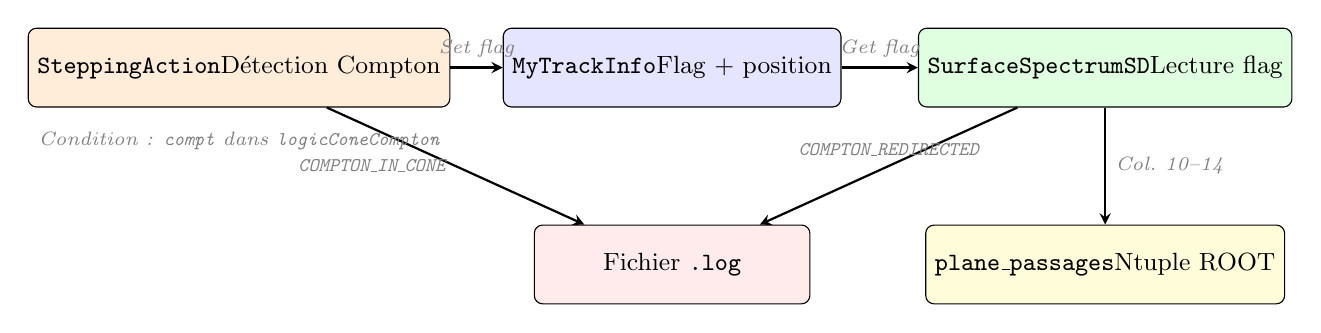
\begin{tikzpicture}[
  box/.style={draw, rounded corners=3pt, minimum height=1cm, minimum width=3.5cm,
              text centered, font=\small},
  arrow/.style={->, >=stealth, thick},
  note/.style={font=\scriptsize\itshape, text=gray},
]

% Boîtes
\node[box, fill=orange!15] (step) at (0,0) {\texttt{SteppingAction}\\D\'etection Compton};
\node[box, fill=blue!10]   (info) at (5.5,0) {\texttt{MyTrackInfo}\\Flag + position};
\node[box, fill=green!12]  (sd)   at (11,0) {\texttt{SurfaceSpectrumSD}\\Lecture flag};
\node[box, fill=yellow!15] (nt)   at (11,-2.5) {\texttt{plane\_passages}\\Ntuple ROOT};
\node[box, fill=red!8]     (log)  at (5.5,-2.5) {Fichier \texttt{.log}};

% Flèches
\draw[arrow] (step) -- node[above, note] {Set flag} (info);
\draw[arrow] (info) -- node[above, note] {Get flag} (sd);
\draw[arrow] (sd)   -- node[right, note] {Col.\ 10--14} (nt);
\draw[arrow] (step) -- node[left, note] {\texttt{COMPTON\_IN\_CONE}} (log);
\draw[arrow] (sd)   -- node[above, note] {\texttt{COMPTON\_REDIRECTED}} (log);

% Annotation processus
\node[note, anchor=north] at (0, -0.7) {Condition : \texttt{compt} dans \texttt{logicConeCompton}};

\end{tikzpicture}
\end{center}


% ===================================================================
%  9. COMPATIBILITE
% ===================================================================
\section{Compatibilit\'e et remarques}

\begin{itemize}[nosep]
\item \textbf{Multi-thread :} le log dans \texttt{SteppingAction} est prot\'eg\'e
      par \texttt{G4AutoLock}. Les compteurs statiques dans \texttt{SurfaceSpectrumSD}
      sont thread-local (\texttt{static} dans une fonction membre appel\'ee par thread).
\item \textbf{Ntuple :} les colonnes 0--9 sont inchang\'ees ;
      les fichiers ROOT existants restent lisibles.
      Les nouveaux fichiers auront 15 colonnes au lieu de 10.
\item \textbf{Autres plans :} ScorePlane2, 3 et 5 ne sont pas modifi\'es.
      Pour les instrumenter de fa\c{c}on analogue, il suffirait de r\'epliquer
      la lecture du \texttt{MyTrackInfo} dans les SD correspondants.
\item \textbf{Performances :} impact n\'egligeable ---
      un test de cha\^ine (\texttt{=="compt"}) et un cast statique par step.
\item \textbf{Recompilation :} seuls les 5 fichiers list\'es doivent \^etre remplac\'es.
      Un \texttt{make} incr\'emental suffit.
\end{itemize}


\end{document}
